
\documentclass[a4paper,12pt]{scrbook}
\usepackage{amsmath,amssymb,amsthm}
\usepackage{fancyvrb}
\usepackage{parskip}
\usepackage{lastpage}
\usepackage{verbatim,boxedminipage,enumitem}
\usepackage{ifthen}
\usepackage{color,graphicx}
\usepackage{pgf}
\usepackage{longtable}
\usepackage{upquote}
%\usepackage[all]{xy}
\usepackage{tobiShell}
\usepackage{tikz}
\usetikzlibrary{automata}
\usetikzlibrary{arrows}
\usepackage{pgf,pgfarrows,pgfnodes}
\usepackage{pgfplots}
\usepackage{circuitikz}
\usetikzlibrary{circuits}
\usetikzlibrary{circuits.logic.US}
\usepackage{mymath}
\usepackage{python}
%------------------------------------------------------------------
% Verbatim for console window - single line frame, no line numbers
%------------------------------------------------------------------
\DefineVerbatimEnvironment%
 {console}{Verbatim}
 {frame=single}

%--------------------------------------------------------
% Remove the vertical spacing before and after Verbatim.
%--------------------------------------------------------
\usepackage{atbeginend}
\BeforeBegin{console}{\mbox{}\\ \begin{minipage}{\textwidth}\vspace{3pt}}
\AfterEnd{console}{\vspace{4pt} \end{minipage} \\ }

\begin{document}
\thispagestyle{empty}

\begin{center}
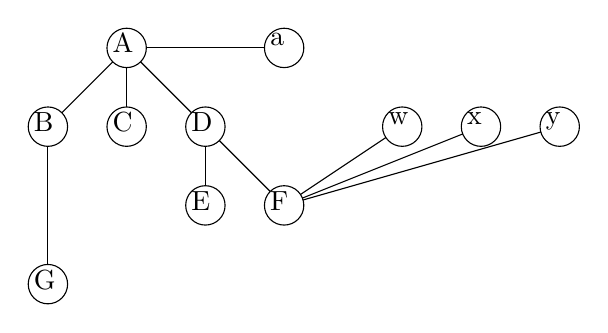
\begin{tikzpicture}
\draw[black] (1.0, 0) circle (0.25);\draw (1.0,0) node[color=black, inner sep=0cm] {
 
\begin{minipage}[t][0.354cm]{0.354cm}
A
\end{minipage}

};\draw[black] (3.0, 0) circle (0.25);\draw (3.0,0) node[color=black, inner sep=0cm] {
 
\begin{minipage}[t][0.354cm]{0.354cm}
a
\end{minipage}

};\draw[black] (1.0, -1) circle (0.25);\draw (1.0,-1) node[color=black, inner sep=0cm] {
 
\begin{minipage}[t][0.354cm]{0.354cm}
C
\end{minipage}

};\draw[black] (0.0, -1) circle (0.25);\draw (0.0,-1) node[color=black, inner sep=0cm] {
 
\begin{minipage}[t][0.354cm]{0.354cm}
B
\end{minipage}

};\draw[black] (2.0, -2) circle (0.25);\draw (2.0,-2) node[color=black, inner sep=0cm] {
 
\begin{minipage}[t][0.354cm]{0.354cm}
E
\end{minipage}

};\draw[black] (2.0, -1) circle (0.25);\draw (2.0,-1) node[color=black, inner sep=0cm] {
 
\begin{minipage}[t][0.354cm]{0.354cm}
D
\end{minipage}

};\draw[black] (0.0, -3) circle (0.25);\draw (0.0,-3) node[color=black, inner sep=0cm] {
 
\begin{minipage}[t][0.354cm]{0.354cm}
G
\end{minipage}

};\draw[black] (3.0, -2) circle (0.25);\draw (3.0,-2) node[color=black, inner sep=0cm] {
 
\begin{minipage}[t][0.354cm]{0.354cm}
F
\end{minipage}

};\draw[black] (4.5, -1) circle (0.25);\draw (4.5,-1) node[color=black, inner sep=0cm] {
 
\begin{minipage}[t][0.354cm]{0.354cm}
w
\end{minipage}

};\draw[black] (6.5, -1) circle (0.25);\draw (6.5,-1) node[color=black, inner sep=0cm] {
 
\begin{minipage}[t][0.354cm]{0.354cm}
y
\end{minipage}

};\draw[black] (5.5, -1) circle (0.25);\draw (5.5,-1) node[color=black, inner sep=0cm] {
 
\begin{minipage}[t][0.354cm]{0.354cm}
x
\end{minipage}

};\draw[black] (0.823223304703,-0.176776695297) to  (0.176776695297,-0.823223304703);
\draw[black] (1.0,-0.25) to  (1.0,-0.75);
\draw[black] (1.1767766953,-0.176776695297) to  (1.8232233047,-0.823223304703);
\draw[black] (1.25,0.0) to  (2.75,0.0);
\draw[black] (0.0,-1.25) to  (0.0,-2.75);
\draw[black] (2.0,-1.25) to  (2.0,-1.75);
\draw[black] (2.1767766953,-1.1767766953) to  (2.8232233047,-1.8232233047);
\draw[black] (3.20801257358,-1.86132495094) to  (4.29198742642,-1.13867504906);
\draw[black] (3.23211917272,-1.90715233091) to  (5.26788082728,-1.09284766909);
\draw[black] (3.24038098691,-1.93131971803) to  (6.25961901309,-1.06868028197);
\end{tikzpicture}

\end{center}

\end{document}
